%%%%%%%%%%%%%%%%%%%%%%%%%%%%%%%%%%%%%%%%%
% University Laboratory Report mainly used in programming
% LaTeX Template
% Version 1.0 (12/9/16)
%
% Author: Chaoyang Liu
% E-mail: chaoyanglius@outlook.com 
% (https://chaoyangliu.cc)
%
% License:
% CC BY-NC-SA 3.0 (http://creativecommons.org/licenses/by-nc-sa/3.0/)
%
%%%%%%%%%%%%%%%%%%%%%%%%%%%%%%%%%%%%%%%%%

\documentclass[hyperref,UTF8]{ctexart}
\usepackage{listings} % Required for setting of code block
\usepackage[colorlinks,linkcolor=black]{hyperref}
\usepackage{color}
\usepackage{graphicx} % Required for the inclusion of images
\usepackage{varwidth} % Required for 
\usepackage{float}

\usepackage{graphicx} % Required for the inclusion of images
\usepackage{natbib} % Required to change bibliography style to APA
\usepackage{amsmath} % Required for some math elements 

%\renewcommand{\labelenumi}{\alph{enumi}.} % Make numbering in the enumerate environment by letter rather than number (e.g. section 6)
\CTEXsetup[format={\Large\bfseries}]{section}
%----------------------------------------------------------------------------------------
% SETTING OF CODE BLOCK
%----------------------------------------------------------------------------------------
\lstset{ % 代码高亮
	backgroundcolor=\color{white},   % choose the background color
	basicstyle=\footnotesize\ttfamily,        % size of fonts used for the code
	columns=fullflexible,
	numbers=left,                    % where to put the line-numbers; possible values are (none, left, right)
	numbersep=0.5em,		% how far the line-numbers are from the code
	breaklines=true,                 % automatic line breaking only at whitespace
	captionpos=t,                    % sets the caption-position to bottom
	tabsize=4,
	frame = single,
	framexleftmargin=2em,
	commentstyle=\color{green},    % comment style
	escapeinside={\%*}{*)},          % if you want to add LaTeX within your code
	keywordstyle=\color{blue},       % keyword style
	stringstyle=\color[rgb]{0.58,0,0.82}\ttfamily,     % string literal style
	rulecolor=\color{black},
	% identifierstyle=\color{red},
	language=c++,
	showtabs = false,
	showstringspaces = false,
	showspaces = false,
}

%----------------------------------------------------------------------------------------
% PDF INFORMATION
%----------------------------------------------------------------------------------------
% You need to set it in curly brace
% according to your information
\hypersetup{
	pdftitle={title of your document},
	pdfauthor={your name},
	pdfsubject={subject of your document},
	pdfkeywords={key words},
}

%----------------------------------------------------------------------------------------
%	DOCUMENT INFORMATION
%----------------------------------------------------------------------------------------

\title{频域处理:以傅立叶变换为例} % Title

\author{\kaishu 刘朝洋} % Author name

\date{\today} % Date for the report

\begin{document}

\maketitle % Insert the title, author and date

\begin{center}
\begin{tabular}{l r}
专业班级: & 计算机141 \\ % Date the experiment was performed
学生姓名: & 刘朝洋 \\ % Partner names
指导老师: & 杨龙 % Instructor/supervisor
\end{tabular}
\end{center}

% If you wish to include an abstract, uncomment the lines below
\begin{abstract}
该实验报告中主要使用OpenCV库函数对某个图像进行离散傅立叶变换。另外,为了进一步理解离散傅立叶变换的性质,又分别对几何变换后的图像进行傅里叶变换。通过对比实验结果来验证离散傅立叶变换的性质。
\end{abstract}

\pagestyle{plain}
%----------------------------------------------------------------------------------------
%	SECTION 1
%----------------------------------------------------------------------------------------

\section{实验目的}

\begin{enumerate}

\item 理解傅里叶变换的原理及方法;
\item 学会使用OpenCV对图像进行傅里叶变换;
\item 理解傅里叶变换的几个性质。

\end{enumerate}
 
%----------------------------------------------------------------------------------------
%	SECTION 2
%----------------------------------------------------------------------------------------

\section{实验内容}

\begin{enumerate}

\item 使用OpenCV库函数对原图像进行傅里叶变换;
\item 将原图像旋转一定角度再进行傅里叶变换,对比变换结果;
\item 将原图像平移一定单位再进行傅里叶变换,对比变换结果;
\item 将原图像缩小一定比例再进行傅里叶变换,对比变换结果;

\end{enumerate}

%----------------------------------------------------------------------------------------
%	SECTION 3
%----------------------------------------------------------------------------------------

\section{实验过程}

\subsection{对图像进行傅里叶变换}

下面是对图像进行傅里叶变换的主要步骤:

\begin{enumerate}

\item 扩展原图像已获得DFT处理的最佳大小;

\begin{lstlisting}
// Expand the image to an optimal size
	int r = getOptimalDFTSize(transformedSrc.rows);
	int c = cvGetOptimalDFTSize(transformedSrc.cols);
	copyMakeBorder(transformedSrc, padded, r - transformedSrc.rows, 0, c - transformedSrc.cols, 0, BORDER_CONSTANT);
\end{lstlisting}
\item 将图像转换为复数形式,并将像素的类型转换为\lstinline{float};

\begin{lstlisting}
// Make place for both the complex and the real values
	Mat planes[] = { Mat_<float>(padded), Mat::zeros(padded.size(), CV_32F) };
	Mat complexSrc;
	merge(planes, 2, complexSrc);
\end{lstlisting}

\item 调用OpenCV库函数对扩展后的图像进行傅里叶变换;
\begin{lstlisting}
// Make the Discrete Fourier Transform
	dft(complexSrc, complexSrc);
\end{lstlisting}
\item 将傅里叶变换结果转为模长,得到变换的频谱图;

\begin{lstlisting}
// Transform the real and complex values to magnitude
	split(complexSrc, planes);
	Mat mag(transformedSrc.size(), CV_32F);
	magnitude(planes[0], planes[1], mag);
\end{lstlisting}

\item 为了便于观察,将图像进行对数拉伸和均衡化处理。

\begin{lstlisting}
// Switch to a logarithmic scale
	mag += Scalar::all(1);
	log(mag, mag);
// Normalize
	normalize(mag, mag, 0, 1, CV_MINMAX);
\end{lstlisting}
\item 为了便于分析和处理,将频谱原点移到图像中心;

\begin{lstlisting}
	int cr = mag.rows / 2; int cc = mag.cols / 2;
	Mat tl(mag, Rect(0, 0, cc, cr));
	Mat tr(mag, Rect(cc, 0, cc, cr));
	Mat bl(mag, Rect(0, cr, cc, cr));
	Mat br(mag, Rect(cc, cr, cc, cr));

	Mat temp;
	tl.copyTo(temp);
	br.copyTo(tl);
	temp.copyTo(br);

	tr.copyTo(temp);
	bl.copyTo(tr);
	temp.copyTo(bl);

\end{lstlisting}

\end{enumerate}

下面是某图像以及它的DFT结果:

\begin{figure}[H]
\centering
\begin{varwidth}[t]{\textwidth}
\vspace{0pt}
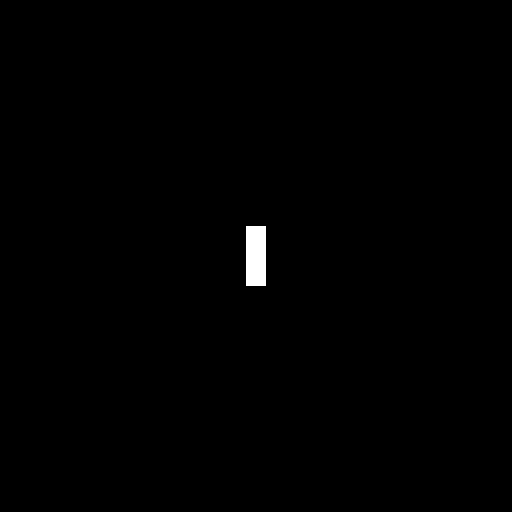
\includegraphics[height=5cm]{rect.png}
\caption{原图像}
\label{fig:rect}
\end{varwidth}%
\quad
\begin{varwidth}[t]{\textwidth}
\vspace{0pt}
\centering
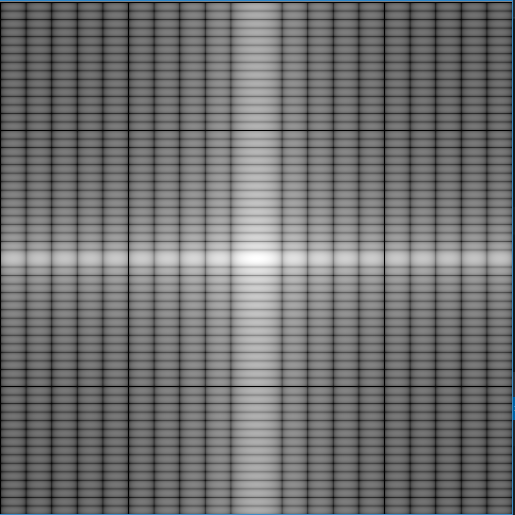
\includegraphics[height=5cm]{rectDFT.png}
\caption{原图像DFT结果}
\label{fig:rectDFT}
\end{varwidth}
\end{figure}


\subsection{DFT的时移性质}


DFT具有时移性质,即对原始图像进行平移变换后,DFT的结果仍保持不变,这一性质可用下面的数学表达式表示:

\begin{equation}
f(x-x_0,y-y_0) \Leftrightarrow F(u,v)e^{j2 \pi (\frac{ux_0}{M} + \frac{vy_0}{N})}
\end{equation}

首先我们需要对图像进行平移操作,通过OpenCV中的仿射变换(Affine Transformations)即可很容易实现。首先要得到变换矩阵,可通过函数\lstinline{getAffineTransform} 得到,只要向该函数传递变换前与变换后的三个点的位置即可产生该变换矩阵。

\begin{lstlisting}
	Point2f s[3] = { Point2f(0, 0), Point2f(1, 0), Point2f(1, 1) };
	Point2f d[3] = { Point2f(x_offset, y_offset), Point2f(1 + x_offset, y_offset), Point2f(1 + x_offset, 1 + y_offset) };
	Mat M(2, 3, CV_32FC1);
	M = getAffineTransform(s, d);
\end{lstlisting}

然后将该变换矩阵传递给函数 \lstinline{warpAffine} 即可。

\begin{lstlisting}
	warpAffine(src, dst, M, src.size(), 1, 0);
\end{lstlisting}

下图\ref{fig:shift}为平移变换之后的图像:

\begin{figure}[H]
\centering
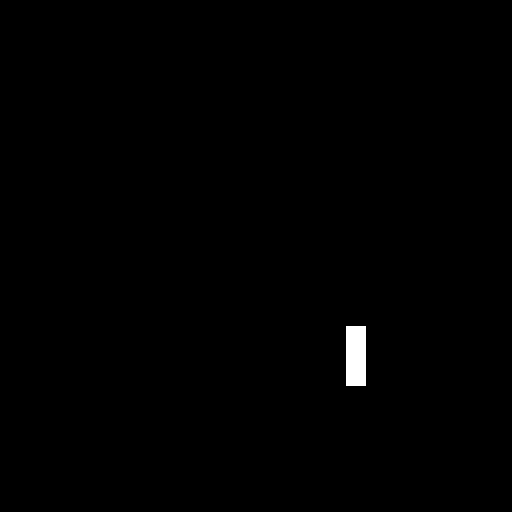
\includegraphics[width=5cm]{shift.png}
\caption{平移变换后的图像}
\label{fig:shift}
\end{figure}

最后,使用前面的相同的处理方法,对平移过后的图像做傅里叶变换,下图\ref{fig:shiftDFT}是DFT结果:

\begin{figure}[H]
\centering
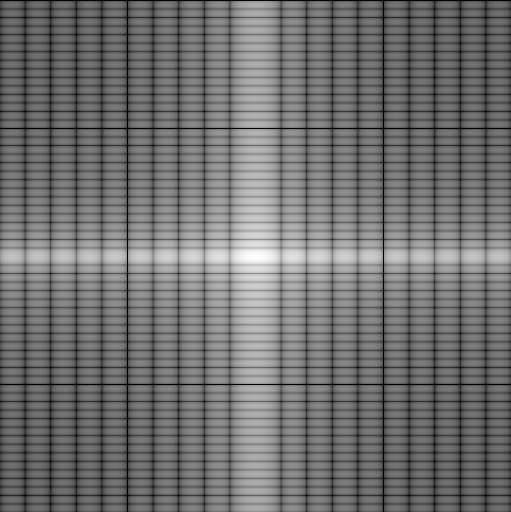
\includegraphics[width=5cm]{shiftDFT.PNG}
\caption{平移变换后图像的DFT结果}
\label{fig:shiftDFT}
\end{figure}

\subsection{DFT的旋转不变性质}

离散傅里叶变换也具有旋转不变性质,数学表达式如下:

\begin{equation}
f(r,\theta + \theta_0) \Leftrightarrow F(\rho ,\varphi + \theta_0)
\end{equation}

OpenCV仿射变换同样可以很容易实现图像的旋转,方法与平移变换类似:

\begin{lstlisting}
	Point center(src.cols / 2, src.rows / 2);
	Mat rotMat = getRotationMatrix2D(center, Rotdegree, 1.0);
	warpAffine(src, dst, rotMat, src.size(), 1, 0);
\end{lstlisting}

下图\ref{fig:rotate}是图像顺时针旋转90 \textdegree 之后的结果:

\begin{figure}[H]
\centering
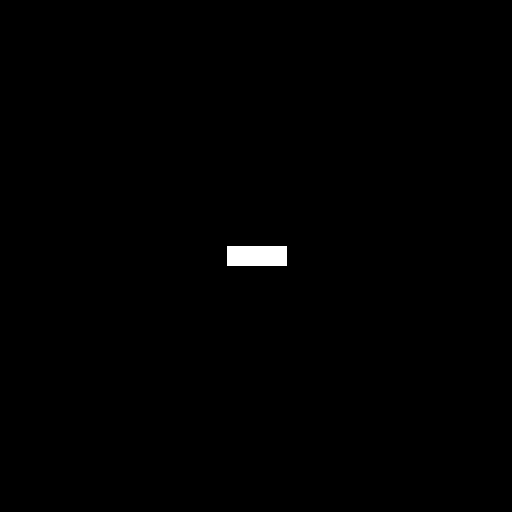
\includegraphics[width=5cm]{rotate.png}
\caption{旋转变换后的图像}
\label{fig:rotate}
\end{figure}

同样,我们需要对旋转后的图像做傅里叶变换,下图\ref{fig:rotateDFT}为DFT结果:

\begin{figure}[H]
\centering
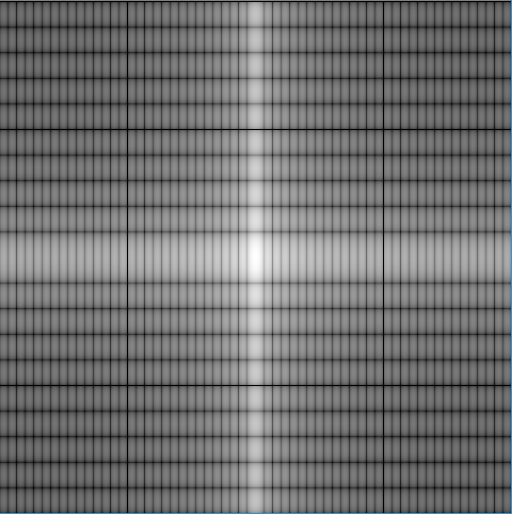
\includegraphics[width=5cm]{rotateDFT.png}
\caption{旋转变换后图像的DFT结果}
\label{fig:rotateDFT}
\end{figure}


\subsection{DFT的比例性质}

离散傅立叶变换的另一个性质是比例性质,数学表达式为,

\begin{equation}
f(ax,by) \Leftrightarrow \frac{1}{ab}F(\frac{u}{a},\frac{v}{b})
\end{equation}

使用仿射变换同样可以很容易实现图像的缩放。

\begin{lstlisting}
	Point2f s[3] = { Point2f(src.cols, 0), Point2f(src.cols, src.rows), Point2f(0, src.rows) };
	Point2f d[3] = { Point2f(Scale * src.cols, 0), Point2f(Scale * src.cols, Scale * src.rows), Point2f(0, Scale * src.rows) };
	Mat M(2, 3, CV_32FC1);
	M = getAffineTransform(s, d);
	Mat tmp = src.clone();
	warpAffine(src, tmp, M, src.size(), 1, 0);
	Mat(tmp, Rect(0, 0, Scale * src.cols, Scale * src.rows)).copyTo(dst);
\end{lstlisting}


接着对图像进行DFT,下图\ref{fig:scaleDFT}是处理结果:

\begin{figure}[H]
\centering
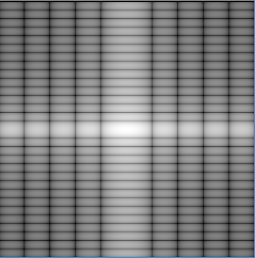
\includegraphics[width=5cm]{scaleDFT.PNG}
\caption{缩小后图像的DFT结果}
\label{fig:scaleDFT}
\end{figure}

%----------------------------------------------------------------------------------------
%	SECTION 4
%----------------------------------------------------------------------------------------

\section{结果与结论}

通过上面的过程,不难发现,无论对图像进行平移、旋转还是缩放,图像的DFT结果仍然保持不变。这与离散傅立叶变换的性质,即平移性质、旋转不变性质以及比例性质,完全吻合。


%----------------------------------------------------------------------------------------


\end{document}